\documentclass[18pt]{beamer}
\usepackage[utf8]{inputenc} % for the umlauts

\beamertemplatenavigationsymbolsempty
%% SLIDE FORMAT

% use 'beamerthemekit' for standard 4:3 ratio
% for widescreen slides (16:9), use 'beamerthemekitwide'

\usepackage{templates/beamerthemekit}
% \usepackage{templates/beamerthemekitwide}

\setcounter{tocdepth}{1}
\usepackage{caption}

%% TITLE PICTURE

% if a custom picture is to be used on the title page, copy it into the 'logos'
% directory, in the line below, replace 'mypicture' with the 
% filename (without extension) and uncomment the following line
% (picture proportions: 63 : 20 for standard, 169 : 40 for wide
% *.eps format if you use latex+dvips+ps2pdf, 
% *.jpg/*.png/*.pdf if you use pdflatex)

%\titleimage{mypicture}

%% TikZ INTEGRATION

% use these packages for PCM symbols and UML classes
% \usepackage{templates/tikzkit}
% \usepackage{templates/tikzuml}

% the presentation starts here

\usepackage[absolute,overlay]{textpos}
%\usepackage[texcoord,grid,gridunit=mm,gridcolor=red, subgridcolor=green]{eso-pic}

\title[BPTI]{BPTI: Projektvorstellung}
\subtitle{Gruppe 03}
\author{Niklas Metz, Felix Bachmann}
\date{07.12.2017}

\institute{}

% Bibliography

\usepackage[citestyle=authoryear,bibstyle=numeric,hyperref,backend=biber]{biblatex}
\addbibresource{templates/example.bib}
\bibhang1em

\begin{document}

% change the following line to "ngerman" for German style date and logos
\selectlanguage{ngerman}

%title page
\begin{frame}
\titlepage
\end{frame}

\section{Idee}
	\subsection{Vorstellung}
		\begin{frame}
			\frametitle{Unsere Inspiration}
			\begin{figure}[H]
				\centering
				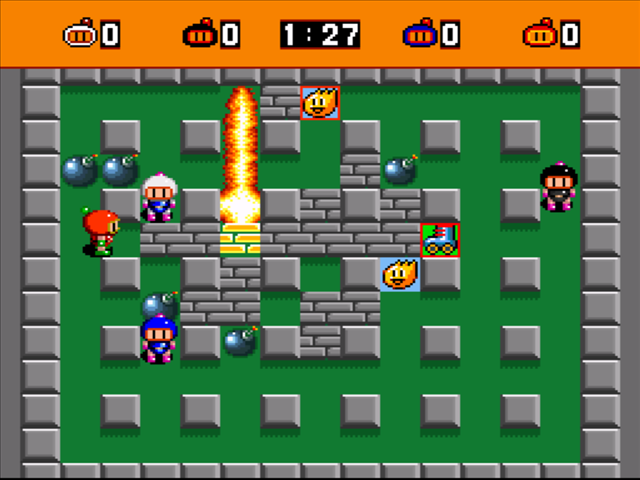
\includegraphics[scale=0.35]{../bomberman.png}
				\centering
				\caption*{Super Bomberman, SNES \newline Quelle: \url{http://hero.wikia.com/wiki/File:Super-bomberman-1-02.png} }
			\end{figure}
		\end{frame}
		\begin{frame}
			\frametitle{Musskriterien}
			\begin{itemize}
				\item vereinfachte Darstellung
				\item Zweispieler-Modus
				\item Bewegung von Spielfiguren
				\item Platzieren und Explodieren von Bomben
				\item Zerstörung der Blöcke, Gegner
			\end{itemize}
		\end{frame}
		\begin{frame}
			\frametitle{Wunschkriterien}
			\begin{itemize}
				\item Sprites
				\item Powerups
				\item bis zu vier Spieler
				\item KI-Gegner
			\end{itemize}
		\end{frame}
	\section{Planung}
		\subsection{Zeitplan}
		\begin{frame}
			\frametitle{Zeitplan}
			\begin{table}[H]
				\centering
				\label{my-label}
				\begin{tabular}{l|l|l}
					Ziel                                      & Verantworliche(r) & Zeitvorgabe  \\
					\hline
					Schaltungsentwurf                         & beide           & bis 15.12.17 \\
					Darstellung des Spielfelds                & Niklas          & bis 22.12.17 \\
					Blockverteilung auf Spielfeld             & Felix           & bis 22.12.17 \\
					Spielfigur - Darstellen, Bewegen          & Felix           & bis 08.01.18 \\
					Spielfigur - Kollision                    & Niklas          & bis 15.01.18 \\
					Platzieren von Bomben                     & Niklas          & bis 15.01.18 \\
					Ticken der Bombe                          & Felix           & bis 18.01.18 \\
					Explosionen - Darstellung                 & Niklas          & bis 26.01.18 \\
					Explosionen - Kollision (Spieler, Blöcke) & Felix           & bis 01.02.18 \\
					Testen, Debugging, Wunschkriterien        & beide           & bis 08.02.18
				\end{tabular}
			\end{table}
		\end{frame}
		
		\begin{frame}
			\frametitle{Danke für eure Aufmerksamkeit!}
			\begin{figure}[H]
				\centering
				
\includegraphics[scale=0.25]{../bomberman_throw.png}
				\centering
				\caption*{\begin{tiny}
						Quelle: \url{https://the-driz.deviantart.com/art/Bomberman-575104646}
					\end{tiny} }
			\end{figure}
		\end{frame}
\end{document}